% Autor: Lukas Deeken
% Letzte Bearbeitung: 01.05.2022

\chapter{Elektromechanische Systeme}

\section{Akkumulator}

\subsection{Zellenauswahl}

Wichtig bei der zellenauswahl ist das stets jede individuelle zelle für sich begutachtet werden muss. es gibt bei den diversen Bauformen und chemischen Zusammensetzungen gewissen Tendenzen welche im folgen erläutert werden. Jedoch ist die Überlappung dieser Eigenschaften in der Regel so groß das sich augenscheinlich vollkommen unterschiedliche Zellen für einen ähnlichen Einsatzzweck eignen.

\subsubsection{Vergleich der Speicherarten}

im nachfolgenden wird die zuerst die Energie berechnet die ein klassiches Formula Studentfahrzeug bei einem typischen bremsvorgang freisetzt und damit die enrgie die mann mindestens speichern können müsste um mit der speciherform auf sinnvolle art und weise eine rekuperation umszusetzten. Im anschluss wird diese energie in eine ungefähre masse an speicherelementen umgesetzt um zu zeigen inwiefern sich diese form der enrgiespeicherung für den einsatz eignet. im nachfolgenden wird die masse an speciherelementen bestimmt um 6 Kwh energie zu speichern da dies der typsiche energieverbrauch eines formula student fahrzueuges im Endurance ist. dieser wert wurde im rahmen eines benchmarkings mit den fahrzeuigen anderer teams über die letzten jahre 2016 bis 2019 errechnet.

Im folgenden errechnen wir die Energie welche bei einem durchschnittlich Bremsvorghang eines formula student fahrzeuges aufgenommen werden müsste. 

\begin{equation}
\glsc{symb:E_kin} = \dfrac{1}{2} * \glsc{symb:m} * \glsc{symb:v}^2
\end{equation}

\glsc{symb:m} = 220Kg
\\
\glsc{symb:v}\textsubscript{Start} = 30m/s
\\
\glsc{symb:v}\textsubscript{end} = 5m/s
\\
\glsc{symb:E_kin} * \glsc{symb:mu} = 74,8kJ
\\

Physikalische Speicher (Kondensatoren)
\\
	Kondensatoren erreichen ein sehr hohes Leistungsgewicht, zeichnen sich jedoch durch eine geringe Energiedichte aus, sowohl gravimetrisch als auch volumetrisch. daher eignet sich diese Form der Energiespeicherung nur um kurzfristige transienten zu glätten aber nicht um gar ganze Bremsvorgänge an Energie zu speichern.\\
	Der Kondensator mit der höchsten energiedicht welcher bei Würth Elektronik verfügbar ist erreicht 3600J/Kg. Somit würde man ca. 20Kg dieser Kondensatoren brauchen um damit effektiv rekuperieren zu können. Bei einem Gewicht für die akuzellen alleine im TY22 von ca. 30,7Kg ergibt sich das der superkondensator nach akltuellem stand keine sinnvoll einsetzbare technologie darstellt.
\\
Thermische Speicher (Salzakkumulator)
\\
	sind im rahmen der formula student verboten Stand 2022, daher wird hier nicht weiter auf diese form des energiespeichers eingegangen
\\
Mechanische Speicher (Schwungrad)
\\
	Zeichnung sich durch relativ gute energiedichte als auch leistungdichte aus und bilden damit wahrscheinlich am ehesten eine realistische form des kurfristigen speichers für ein formula student fahrzeug. Jedoch sind solche systeme sehr komplex sowohl mechanisch, elektrisch als auch regelungstechnisch im vergleich zu den anderen systemen. Die lagerung und sichere unterbringung des schwungrades in einem formel fahrzeug birgt große technische herausforderungen
\\
Chemische Speicher (Klassische Akkuzelle)
\\
	Der typische im Rahmen der formula studnet von allen teams eingesetzte energiespeicher. In der verfügbaren bandbreite findet man so ziemlich das optimum an leistungs als auch energiedichte.

\subsubsection{Runde vs Pouch vs Prismatische Zellen}
%tabelle
(
	Puch zelle

in der regelung höhere packungsdichte möglich damit höherte volumetrische enrgie und lkeistungsdichte
in der regel weniger zellen weniger als 300 manschmal sogar nur 150
weiches gehäuse ist leicht zu beschädigen, bedarf vorischtiger umgang 
aufblähen beim laden und entladen muss bei konstruktion berücksichtigt werden sonst platzenb der zellen möglich


Rundzelle

geringere fertigungstoleranzen durch serienfertigung idr kein matching erforderlich
hoher grad an standardisierung damit folgen mechanische austauschbarkeit und gute marktverfügbarkeit
Hartes gehäuse damit geringe wahrscheinlichkeit von penetrastion durch spitze objekte
bedarf in der regel sehr vieler zellen 600 und mehr, daher hohe mechanische komplexität

Prismatische Zellen

vorgefertigtes paket aus rund oder pouchzellen
sehr wenige zellen kleiner 150
sehr geringe mechanische komplexität da das paket in der regel mit elektrischen und mechanischen anbindungspunkten kommt meist sind auch schon temperatur sensoren integriert
meist jedoch sehr schwer aufgrund der ausrichtung auf industrielle bedürfnisse


Im rahmen des TY22 haben wir uns für den einsatz von rundzellen entschieden da diese nach unserem kenntnisstand gravimetrisch die höchste energiedichte liefern wir uns langfristig auf ein konzept festelgen wollten und so bei einsatz einer neuen akkuztelle nur gerinfügige änderungen an dem akku machen müssen sofern das 18650 format weiterhin populär bleibt. Außerdem war dies im rahmen der lieferschwierigkeiten im bereich der akuzellen im jahr 2021 die beste option um tatsächlich auch an akkuzellen für den bau des fahrzeuges zu kommen
)

\subsubsection{Zellchemie und Rekuperation}

Im folgenden eine tabellarische gegenüberstellung von \acfirst{LiFePo4} zellen und \acfirst{Li-ion} Zellen. Diese Tabelle basiert auf einer Sichtung von mehr als 30 verschiedenen Akkuzellen welche im rahmen des Projektes auf ihre Eignung für den Einsatz im Fahrzeug geprüft wurden. Liion umfasst dabei ein konglomerat aus diversen zellchemien welches eigentlich auch lifepo4 mit einschließt. Zur vereinfachung des vergleiches wurden alle liion chemieen mit einem typ. arbeitsbereich von 3-4,2 hierunter zusammengafasst. Die hierbei aufgrund der hohen löeistungsdichte am häufigsten vertretene Chemie ist LiNiMnCoO2



In der analyse ergibt sich das bild das sich \acfirst{LiFePo4} zellen für ein konzept mit hohem rekupoerationsanteil aber niederiger gesamtkapazität eignet während sich liion zellen für ein konzepot mit niedrigerem rekuperationsanteil und hoher gesamtkapazität eignen. Weiterhin muss hier berücksichtigt werden das Lifepo4 zellen meist ein niederigers temperaturmlimit beim laden als beim entladen haben was im betrieb zu einem vorzeitigen ausfall der rekuperation durch zu hohe akkutemperaturen führten kann. daher ist das temperatur managment hier von besoinderer bedeutung.

Das konzept mit hohen rekuströmen ist nur beim AWD Fahrzeug sinvoll anwendbar da hier auch die gesamte bremsenergie, abzüglich der verlsute im antriebsstran und einiger spitzenlasten welche die mechanische bremsanlage abfangen muss, verfügbar ist. Aufgrund der hohen komplexität des AWD systemes wurde beim TY22 auf ein 2WD System gesetzt. Daher ist der einsatz von konkret LiNiMnCoO2 zellen am ehesten sinvoll.

\subsubsection{Temperaturmodell der Zelle}

Auf Basis der Masterarbeit Experimentelle Untersuchung von Batteriesystemen im simulierten niedrigen Erdorbit von Agnes Klein an der Universität Stuttgart konnte ich ein simples thermisches modell der akkuzelle in einer excel tabelle ersytellen. Bei dieser arbeit wurde unter anderem die akkuzellen des types VTC6 innerhalb einer thermnal vakuum kammer betrieben und die thermischen paramter der zelle ermittelt. In folgender Grafik finden sie die dabei ermittelten parameter.

\begin{figure}[h]
	\centering
	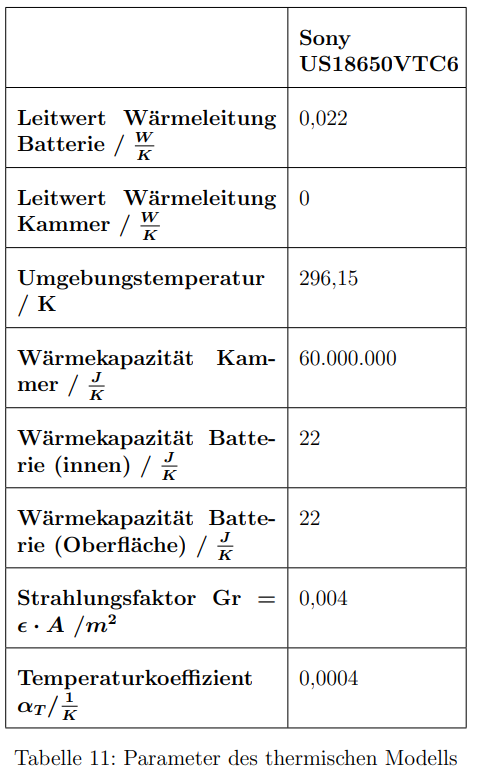
\includegraphics[width=0.4\linewidth]{bilder/Parameter_thermisches_modell_VTC6}
	\caption{}
	\label{fig:parameterthermischesmodellvtc6}
\end{figure}


Damit ergibt sich folgendes Modell.

\begin{equation}
	\glsc{symb:T_celli+1} = (\glsc{symb:I_cell}^2 * \glsc{symb:R_cell} - \glsc{symb:G_th} * (\glsc{symb:T_celli} - \glsc{symb:T_u}) - \glsc{symb:G_r} * \glsc{symb:SBoltz} * (\glsc{symb:T_celli} - \glsc{symb:T_u})^4) * \dfrac{1}{\glsc{symb:C_B} * \glsc{symb:m_Cell}} + \glsc{symb:T_celli}
\end{equation}

Mit diesem Modell ergeben sich folgende Kurvenverläufe für eine Auswahl Entladeströmen

\begin{figure}[h]
	\centering
	\includegraphics[width=0.7\linewidth]{bilder/temperatur_über_energie_vtc6_thermo_modell}
	\caption{}
	\label{fig:temperaturuberenergievtc6thermomodell}
\end{figure}

Mithilfe der folgenden Grafik von der Universität BRNO (MATEC Web of Conferences 313, 00045 (2020)) können wir einen Plausibilitätscheck durchführen. Wir haben hier Messdaten von der Sony VTC6. hierbei sind jedoch die Testbedingungen unbekannt. Als grobe Abschätzung sollte dies jedoch ausreichen

\begin{figure}[h]
	\centering
	\includegraphics[width=0.7\linewidth]{"bilder/Messdaten_VTC6_ temperatur kapazität spannung"}
	\caption{}
	\label{fig:messdatenvtc6-temperatur-kapazitat-spannung}
\end{figure}

Wir sehen das das erstellte modell für den 10A graph um ca. 3°C abweicht. Weiterhin sehen wir das bei der 20A linie die 90°C ca. 0,5Ah früher erreichen. Diese Abweichungen nicht insignifikant, zeigen jedoch das unser modell eher zu hohe als zu niedrige temperaturen ausgiebt was für die zuverlässigkeit des fahrzeuges positiv ist da eine auslegung der kühlung mit diesem modell wahrscheinlich zu einer überkühlung und damit zu einem zu hohen gewicht des kühlsystemes führt was für das erste fahrzeug kein sonderliches problemn darstellt. Die abweichung dürfte darauf zurückzuführen sein das die modellparameter im vakkum ermittelt worden und insofern wärmeübertragung durch konvektion etc. nicht berücksichttigt werden konnte. Um diesem sachverhgalt weiter auf die gründe zu gehen wurde im anschluss eine Simulation mit ansys fluent durchgeführt.

\begin{figure}[h]
	\centering
	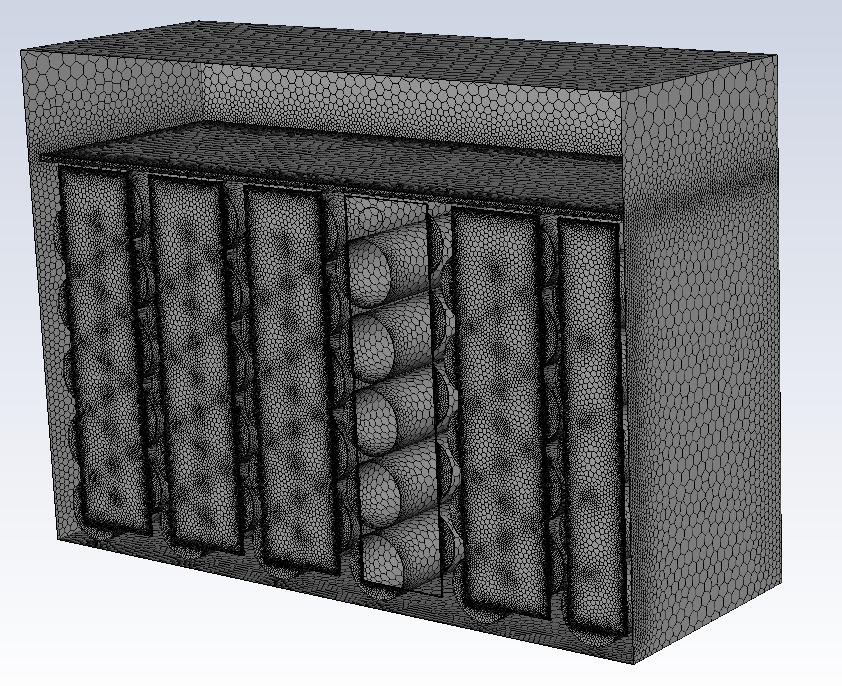
\includegraphics[width=0.7\linewidth]{bilder/Accu_Sim_therm_7_2A_45min_simple_mesh}
	\caption{}
	\label{fig:accusimtherm72a45minsimplemesh}
\end{figure}

\begin{figure}[h]
	\centering
	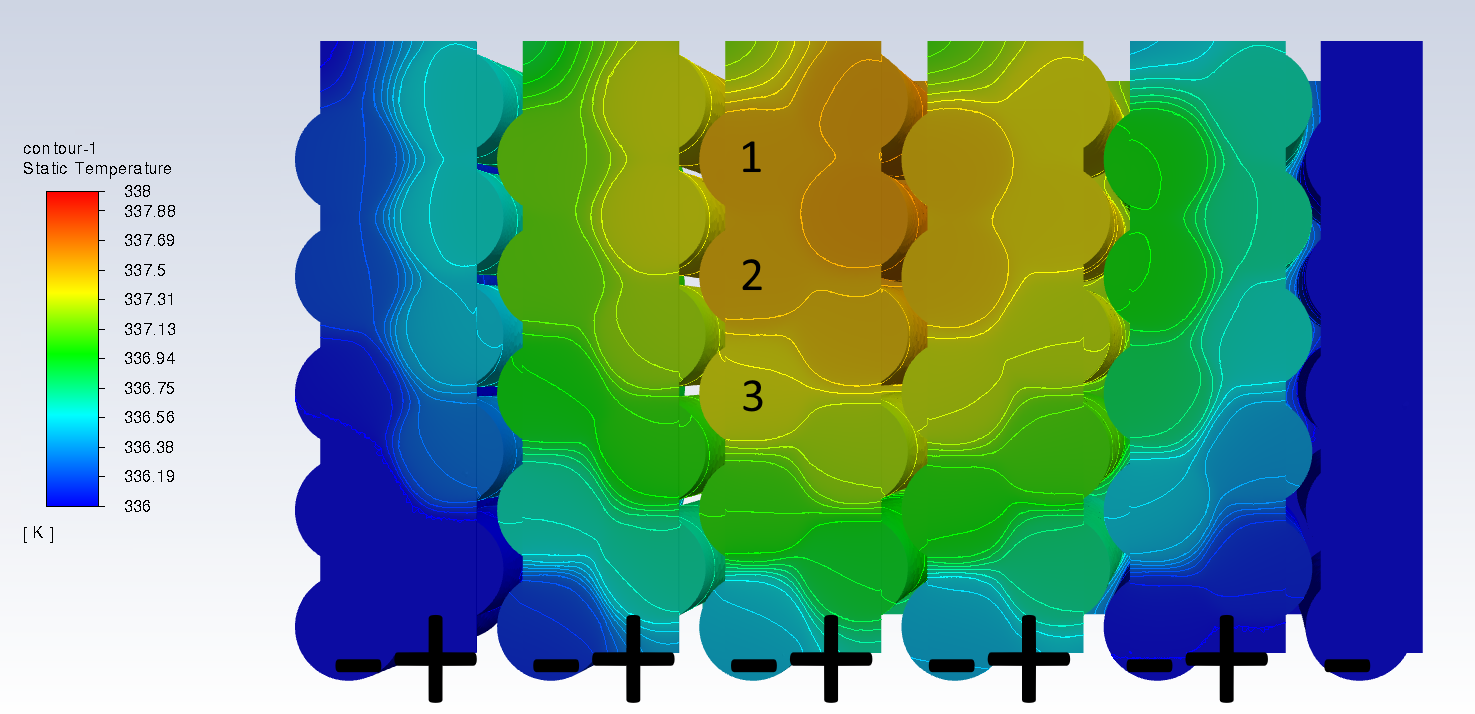
\includegraphics[width=0.7\linewidth]{bilder/Accu_Sim_therm_7_2A_45min_simple}
	\caption{}
	\label{fig:accusimtherm72a45minsimple}
\end{figure}

In dieser simulationb wurde ein gesamter akkustack in seinem gehäuse simuliert. dabei wurde mit einem konstanten strom von 7,2A simuliert. Dieser strom ergibt sich aus der rundenzeitsimulation siehe sectrion. Die Simulation wurde für 32min laufen gelassen um eine gesamtes endurance darzustellen. Ziel der simuzlation ist es die effekte der konvektion zu berücksichtigen aber auch zu sehen in wiefern sich die zellen gegenseitig beeinflussen. Allerdings wurden auch diverse vereinfachungen getroffen insofern das die akkuzellen sich uniform aufwäremn. In der realität dürfte man am negativen pol der akuzelle eine deutlich höhere temperatur feststellen könne als auf der positiven seite. weiterhin wurden diverse teile wie die elektrische isolierung etc. weggelassen da dies den simulations aufwand sonst erheblich vergrößert hätte und die simulation so schon 2 tage benötigt hat. zur analyse, wir sehen nach der simulationszeiot eine hot spot temperature von 64,85°C und eine niedrigste temperatur von 62,85°C. In dieser hinsicht stimmt die ansys simulation eher mit der 10A kurve aus unserem modell zusammen als mit den messdaten. Zusammengefasst stellt man fest das definitiv weitere arbeit in diesem themenbereich von nöten wäre um zu einer optimalen lösung zu kommen dies jedoch aufgrund des engen zeitplanes und des enoremn anderweitigen aufwandes nicht möglich ist.

\subsubsection{Die \glqq Ideale\grqq Akkuzelle}

\subsubsection{Der Stack Aufbau}
Halterkonstruktion
Maintenace Plug design
AMS Slave montage

\subsubsection{Die Busbar}
Busbar material und dicken auswahl
Schweißverfahren


\subsubsection{Der Accumulator Conatiner}

\section{Elektromotor}
Im großen und ganzen gibt es für die Auswahl des Elektromotors 4 verschiedene in der Formula Student allgemein anerkannte Lösungen. Diese werden nachfolgend erläutert.

\subsection{Emrax}
Beim Emrax Motor handelt es sich um eine Axial Flux Permanent erregte synchron Maschine PMSM. zusammenfassend sind die emrax motoren sehr flacj haben aber einen großen durchmesser. Sie zeichnen sich durch ein hohes drehmoment und damit verhältnismäßig niedrige drehzahlen aus, im bereich von 7-8K RPM. Sie sind nur in recht großen formaten und damit großen leistungen erhältlich so das ein 1 oder 2 motoren antriebskonzept realisierbar ist. Außerdem handelt es sich hierbei um eine reine kauflösung. 

\subsection{AMK}
Die AMK motoren sind radial flux PMSM. Sie sind insofern eher lang und haben kleine druchmesser. Die bauform gleicht insofern eher dem klassischen elektromotor. Sie zeichnen sich durch extrem hohge drehzahlen aus, oberhalb der 20k und damit durch eine enorme leistungsdichte. Sie sind in eher kleinen leistungsdichten zu bekommen so das beinahe nur ein Allrad antrieb sinnvoll umsetzbar ist. Auch hierbei handelt es sich um eine reine kauflösung. 

\subsection{Fischer}
Die Motoren von fischer sind im großen und ganzen gleichzusetzten mit den amk motoren. der große unterschied ist das hier das gehäuse selbst designt werden muss und alle teile selber gefertigt werden müssen. Die stellt große herausfordferungen die fertigungstechnik da es sich dabei auch um 5 achs gefräst6e titanteile handelt. 

\subsection{Selbstbau}
Der selsbtbau ist quais die nächste entwicklungsstufe nach dem fischer motor. Num gilt es nicht nur den motor selber zu fertigung sondern auch die gesamte vorauslegung zu machen. es gibt nur wenige teams die einen selbstbau wagen, und noch werniger die es erfolgreich umsetzten.

\subsection{Entscheidungsfindung}

Die Entscheidung ist an diesem Punkt sehr einfach. Im rahmen dieser projektabreit entsteht der erste e antrioerb aus dem hause baltic racing. damit kommen enrom viele große heruasforderung. das heißt man sollte entweder die einfachste oder die nächst einfachste Lösung nehmen um am ende zu dem ziel des fahrenden autos zu kommen. Und da sich nur der emrax motor effektic für einen zwei rad antrieb eignet ist es der emrax motor gewotrden.

\section{Wechselrichter}
Der wechselrichter wird benötigt um den motor sauber anzusteuern. Ziel ist es aus gleichstrom aus dem akku einen Frequenz und amplituden regelbaren strom zu erzuegen mit dem der motor kontrolliert werden kann. Hier gibt es auch wieder diverse hersteller die im folgenden verglichen werden sollen

!!!Tabelle!!!

\section{Kabelbaum}
Die Entwicklung des Kabelbaumes erfolgt in der regel recht früh im entwicklungsprozess und zieht sich recht lange, da fast jede änderung an den elektrischen systemen auch eine änderung am kabelbaum nachsichzieht. Der kabelbaum lässt sich bei einem elektrofahrzeug iun mehrere funktionsgruppen unterteilen. Einmal haben wir den Datenbuss zur kommunikation der Steuergeräte im Fahrzeug. In unserem fall ist das ein CAN Bus. Dann den sogenannten Shudown circuit zur absicherung der systeme bzw. einleiten eines sicheren zusatendes in dem fall das ein fehler auftritt. Weiter gibt es die gruppe der Hochvolt kabel dies umfasst leistungsführende leiter für akku inerter und Motor als auch HV signalleiter für z.b. die TSMP. Dann haben wir noich die LVS Versorgung für alle systeme im Fahzeug. Dann gibt es den Sensor baum dieser umfasst die versorgungs als auch datenleitungten für jegliche sensorik im fahrzeug  Abschließend gibt es noch alles andere was sich nicht hierunter kategorisieren lässt. Dies umfasst z.b einzelne analoge oder digitale datenleitungeng wie z.b die Ethernet Leitung für den FSG Logger oder die Abzweigleitung des Bremsdruckes für das BSPD. Auf die einzelnen gruppen wird im folgenden detailiert eingegangen.\\
\\
Wichtige generelle Überlegungen beim Kabelbaum sind jegliche Maßnahmen die den Kabelstrang DAU sicher machen. Sprich verpolsichere steckverbinder Belegung der stecker so das ohne verpolschutz kein kapitalschaden eintritt. sauber logische farbcodierung sowohl der Kabel als wenn möglich auch der Steckverbinder sodass beim zusammenbau keine fehler gemacht werden und dies einheitliche am besten über jahre durchgängige durchgeführt.

!!!Liste bzw. übersicht mit Steckverbindern belegungen und farbe!!!

Steckertypen:		
Molex Micro Fit 	both 	Wire Mount	not sealed 	(HV)	2-20
Molex CMC/CMX 		W2B 	Panel Mount	Sealed 		(LV)	28-154
TE HD10/20/30 		both 	both		sealed 		(HV)	3-47
Molex Mizu P 25 	W2W 	Wire Mount	sealed 		(LV)	2-4
Binder Sub M9 		both 	both		sealed 		(LV)	2-8
Binder M12 Power	both	both		sealed		(HV) 	3-4
Würth WRBHD2.54		W2B	Wire Mount	not sealed	(LV)	10
Typ K Stecker
RJ45 stecker

Kabel:
UNITRONIC FD P plus A, 0028660, 4x0.25
White 24V
Brown GND
Green CANH / Signal
Yellow CANL / 5V

Bedia Farben:
White 24V
WhiteXGelb 5V
WhiteXRosa 12V
WhiteXRot 3V (Battery)
Brown GND
Green CANH
Yellow CANL
Blue SDC
BlueXred SDC\textsubscript{end}
BlueXWhite \textsubscript{indicator} (geht nur wenn kabel nicht HV sein muss, sonst blaues HV Kabel)
Violett Sensor-Signal

detakta HV kabel
Red TSMP+ und HV+
Black TSMP- HV-
Blue SDC/Interlock/indication

Coroflex 
HV high power orange
16 \& 25mm\^2

Unitronoic LAN
gelb

Belegung mit MizuP25 Steckern
Can Schwarz 4pin
1 GND (Brown)
2 CANH (Green)
3 24V (White)
4 CANL (Yellow)
Sensoren Weiß 4pin 
1 GND (Brown)
2 5V (Yellow)
3 24V (White)
4 Signal (Green)
Shutdown Schwarz 3Pin
1 SD\textsubscript{in}
2 SD\textsubscript{out}
3 SD\textsubscript{LED}
Servos weiß 3pin
1 Signal (Gelb)
2 GND (Braun)
3 8,3V (Rot)
Brakelight weiß 3pin
1 Signal (Violett)
2 GND (Brown)
3 24V (White)

Belegung Binder 4 Pin
CAN
1 GND
2 CANH
3 12V
4 CANL

Typk nur mit extra TypK Stecker

\subsection{CAN-Bus}
Beim CAN Bus handelt es sich um ein Multi-Master Bus mit zwei normalerweise verdrillten symmetrischen Datenleitungen. Wichtig zu beachten ist das der CAN-Bus immer als linientopologie aufgebaut werden sollte und dabei die anzahl an stichleitungen möglichst klein zu halten ist. Weiterhin muss an enden der Linie ein 120Ohm Wiederstand eigesetzt werden. Für Stichleitungen empfiehlt sich bei Problemen in der busskommunikation ein 4,7kOhm widerstand o.ä. einzusetzen.

\subsection{LVS Versorgung}

Die LVS Versorgung läuft in einer Sterntopologie von der Fusebox aus. Hier befinden sich mittels mikrokontroller überwachte Sicherungen für alle elektrischen Verbraucher. Ausnahmen hiervon sind die versorgung des SDC welcher am LVMS starten muss als auch die versorgung des BSPD welches direkt vom LVMS versorgt werden muss. Die Versorgung der Steuergeräte welche per CAN Bus mit der Fusebox verbunden sind läuft zusammen in einem 4 Ader Kabel mit dem CAN Bus und entspricht daher eher einer Linientopologie. Die Masseleitung laufen an Insgesamt 3 verschiedenen Sternpunkten auf das Chassis zusammen. Einer befindet sich am abnehmbaren Heck des Fahrzeuges, einer rechts hinter der Firewall im Fahrzeug und einer im Vorderbau des Fahrzeuges

\subsection{Sensor Kabelbaum}

Der Sensorkabelbaum besteht aus beinahe ausschließlich 4 Ader Kabeln welche 24V, 5V, GND und ein Signal führen. Diese Kabel laufen sternförmig von jedem der Sensorhubs zu den entsprechenden Sensoren

\subsection{Shutdown Circuit}
\begin{figure}[h]
	\centering
	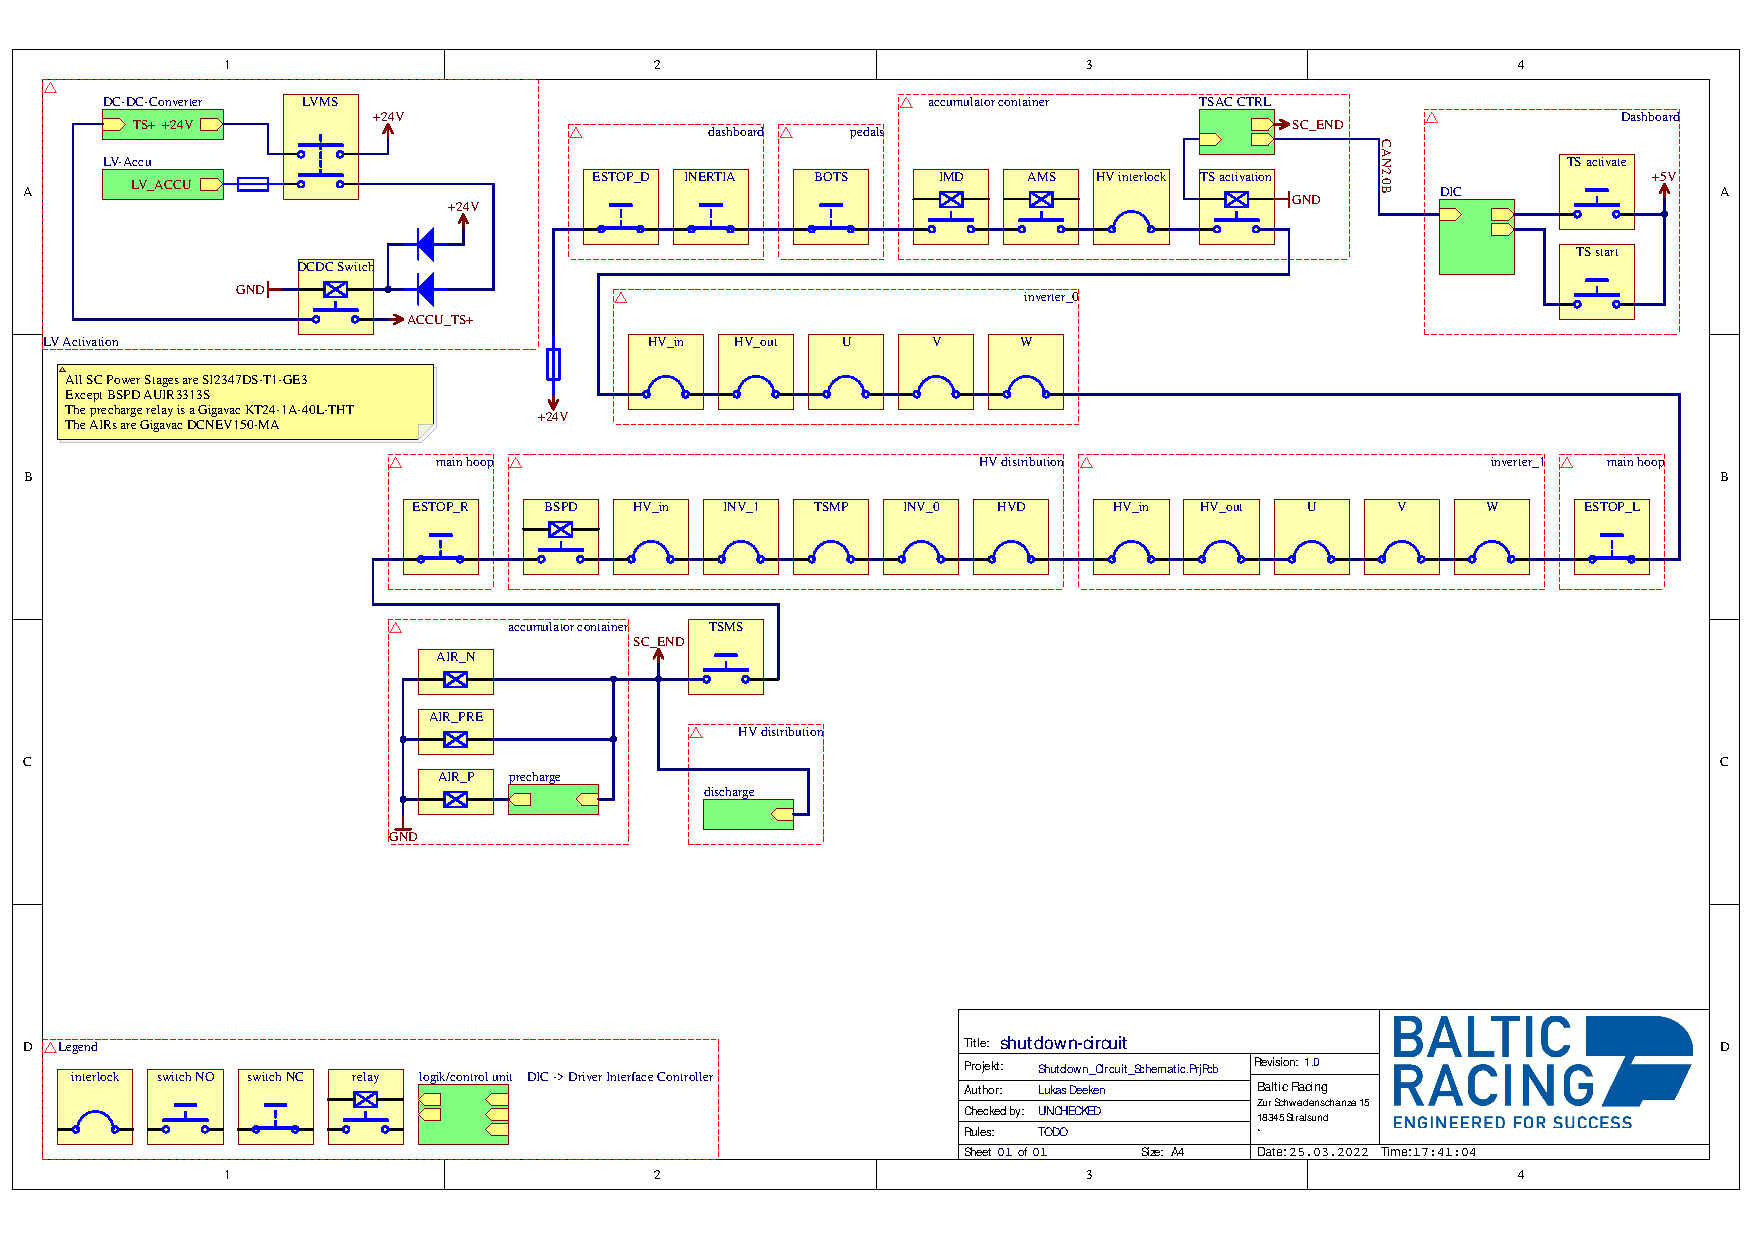
\includegraphics[width=1\linewidth]{bilder/Shutdowncircuit}
	\caption[Shutdown Circuit Schematic]{}
	\label{fig:shutdowncircuit}
\end{figure}

In der obenstehenden Graphic ist der sogenannte shutdown circuit abgebildet. Oben Links befindet sich die Versorgung bzw. der Anfangt des SDC bestehend aus dem Kickstarter für den HVDCDC und der hauptschaltung für das LVMS. Oben rechts befindet sich die TS activation Logik. Im Dashboard des fahrzeuges befinbden sich 2 knopfe, einer um das TS einzuschalten und einer um die Motoren freizuschalten und damit das Losfahren zu ermöglichen. Die kommunikation erfolgt hier über den CAN bus direkt zum AMS Master Auf dem rest des blattes ist von oben nach unten der gesamte shutdowncircuit mit all seinen elementen abgebildet. Am ende des Shutdown circuit befinden sich die AIR welche direkt vom SDC betrieben werden müssen. Weiterhin wird dort das SDCEND Signal abgezweigt welches den ausgangsstatus des SDC abzweigt und z.b dem Discharge bereitstellt.\\
\\
Wichtig beim Shutdowncircuit zu beachten ist das an möglichst vielen stellen stichleitungen eingebracht werden um den SDC an möglichst vielen stellen überwachen zu können. Dies hilft enorm bei der Fehlereingrenzung. Weiter sollter der Querschnitt der Kabel nicht zu dünne gewählt sein. Der Strom im Shutdown Circuit liegt bei ca. 0.24A Da hierrüber ja die AIRs direkt mgeschaltet werden müssen und der SDC hat am ende eine beträchtliche länge im Fahrzeug. 

\subsection{Kabeldimensionierung}
Bei Der Kabeldimensionierung wurden 2 unterschiedliche Ansätze angewandt. Einmal die dimensionierung nach DIN VDE 0298-4 und einmal anhand einer generischen Tabelle. Zweiteres empfiehlt sich eigentlich standardmäßig für so gut wie alle Anwendungen. Ersterer ist hierbei idr nur für soetwas wie die Stromführenden HV Leiter sinnvoll anzuwenden. Die Querschnitberechnung ließe sich mit einem physikalischen Modell noch weiter treiben auf dies wurde jedoch aufgrund des zeitmangels verzichtet.
Folgend ist einmal die bisher verwendete tabelle aufgeführt. Die Quelle der Tabelle war http://www.learn-about-electronics.com/ allerdings ist dies mittlerweile nicht mehr aufzufinden
Bei der Tabelle ist zu beachten das die Ströme für Chassis Wiring verwendet werden. Unter Power Transmission versteht man hier leiter die Mit geringen verlusten z.b in einer industriellen umgebung ströme über lange wege z.b. von Haus zu Haus leiten sollen.
\begin{figure}[h]
	\centering
	\includegraphics[width=0.7\linewidth]{"bilder/Wire thickness"}
	\caption{Leiterquerschnitttabelle}
	\label{fig:wire-thickness}
\end{figure}

Nun soll im Anschluss einmal die Berechnugn der Querschnitte nach DIN VDE 0298-4 (Anhang) dargestellt werden.

Nach 9.4 können wir für ungleichmäßige Ströme den Quadratisdchen Mittelwert zur Leiterquerschnittsbestimmung anstezen. Den Quadratiscvhen mittelwertes des Stromes der Elektromotoren erhalten wir indem wir das mittlere Drehmoment am elektromotor bestimmen, hierfür müssen wir auf die Daten aus der Rundenzeitsimulation zurückgreife, in zukunft empfiehlt es sich die einmal mit den Daten aus dem tatsächlichen fahrzyklus nachzurechnen. Das Drehmoment was wir hier erhalten liegt bei 68,2Nm pro Motor. Im Handbuch des Emrax 208 (Anhang) befindet sich ein Parameter der uns den RMS Strom in A pro NM Drehmoment an der ausgangswelle angiebt. dieser liegt bei 0,8 Nm/A\textsubscript{RMS}. \\
Damit lässt sich ermitteln das der Quadratisdchen Mittelwert des Stromes bei ca. 85,3 A liegt
Nun lässt sich mit hilfe von Tabelle 9.2 der Strom für den Verlegungstyp E (Verlegung wie Motorleiter) für verschiedene Kabelquerschnitte ermitteln Wir ermittlen für 16mm\^2 einen Strom von 80A für 3 belastete Leiter und für 25mm\^2 respektive einen Strom von 101A. Zur sicherheit wurde hier an der stelle auf 25mm\^2 zurückgegriffen, allerdings sollten zukunft durchaus mal versuche mit 16mm\^2 für die Motorleiter unternommen werden da dies zu einer durchaus signifikanten gewichstersparnis führen kann.\\
\\
Für den DC Bus wurde das gleiche vorgehen angewandt. Hier bekommen wir den Strom direkt aus der Rundenzeitsimulation mit 53A. Das ergibt nach Typ E mit 2 belasteten Leitern 10mm\^2 Querschnitt. Jedoch konnten wir keine Steckverbinder finden welcher 10mm\^2 Kabel akzeptiert und ein entsprechendes Rating hat weshalb wir hier auf 16mm\^2 gegangen sind. Auch hier gilt wieder das noch Möglichkeiten der Gewichtsersparnis bestehen.\\
\\
\subsection{Hochvolt Kabelbaum}

\begin{figure}[h]
	\center
	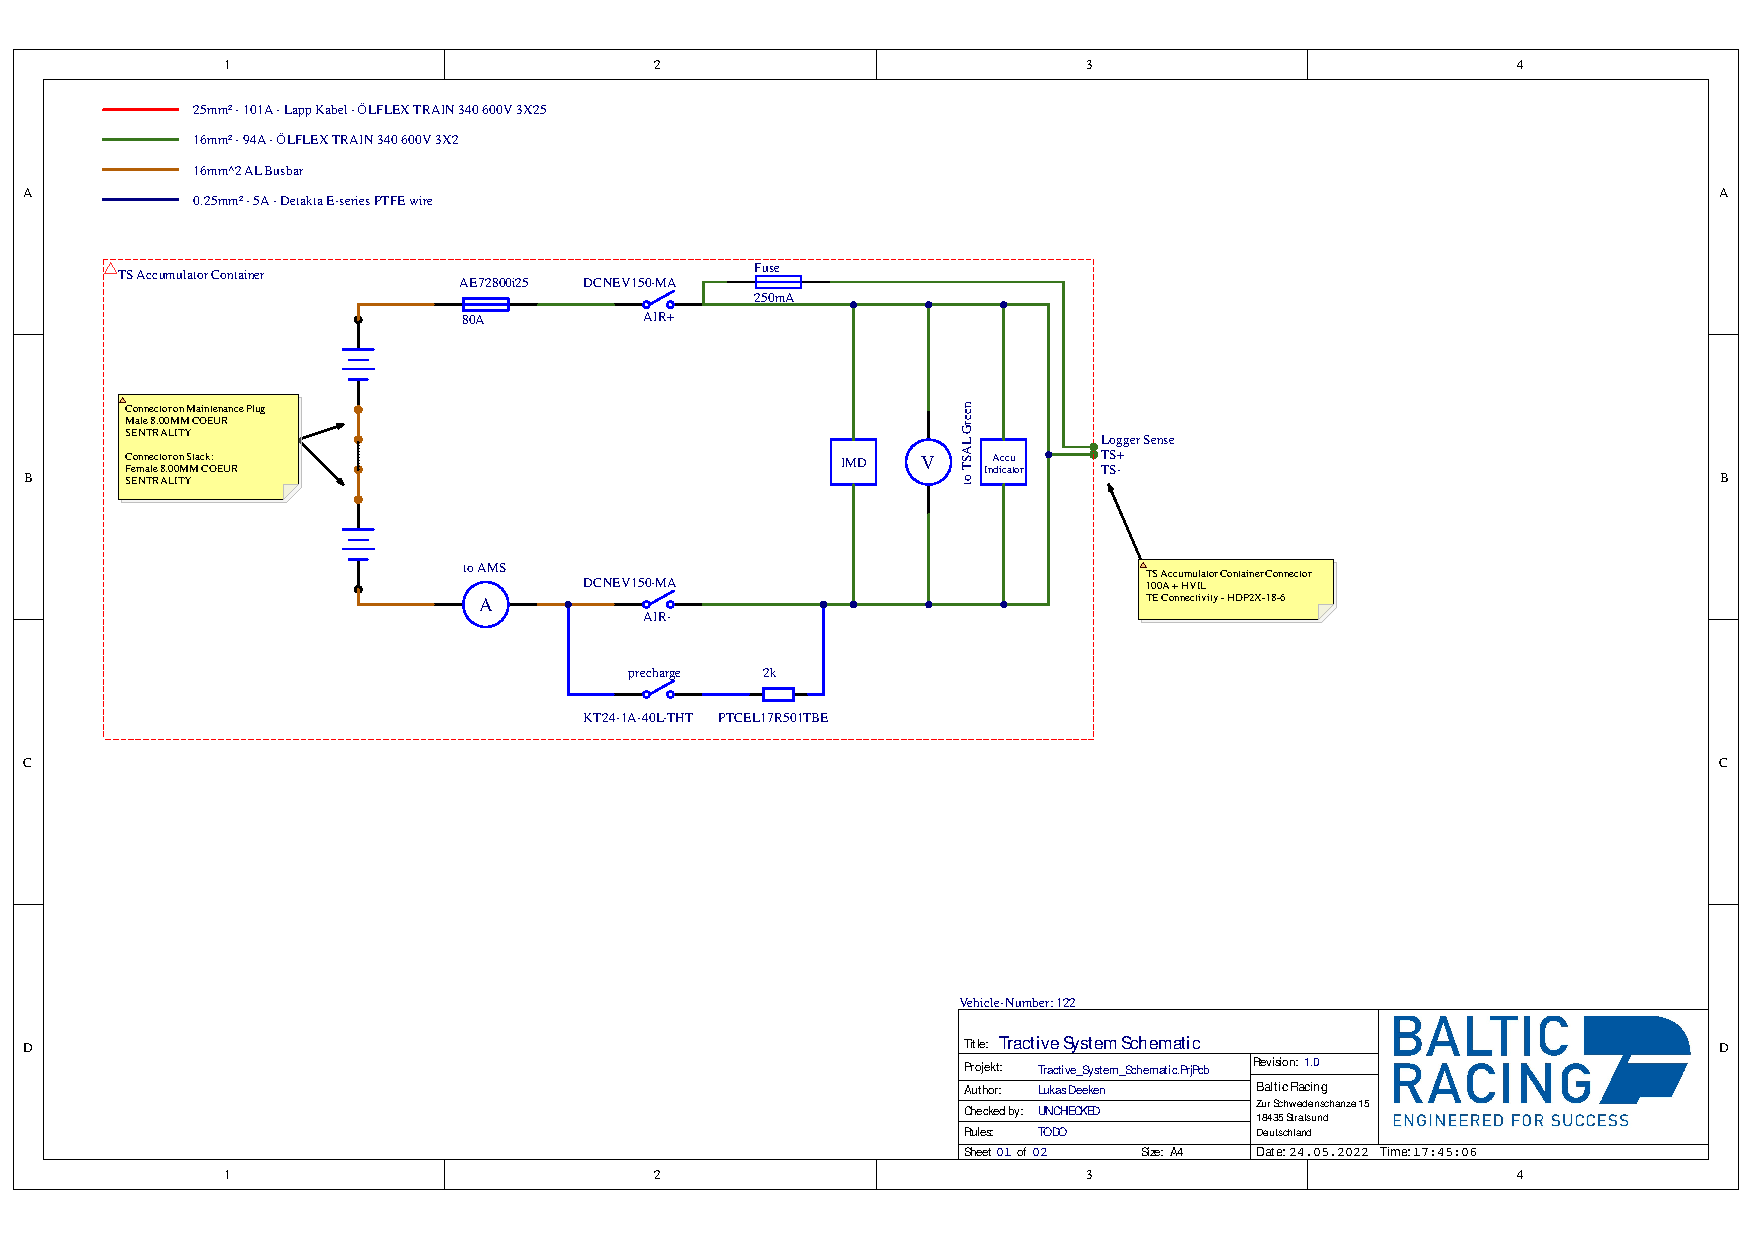
\includegraphics[page=1,width=0.9\linewidth]{bilder/Tractive_System_Schematic_V4.pdf}
	\caption[Tractive System Schematic]{}
	\label{fig:tractivesystemschematic1}
	
	\center
	\includegraphics[page=2,width=0.9\linewidth,]{bilder/Tractive_System_Schematic_V4.pdf}
	\caption[Tractive System Schematic]{}
	\label{fig:tractivesystemschematic2}
	\end{figure}

Der HV Kabelbaum besteht aus 3 Kabelsträngen, einer befindet sich innerhalb des Akkus, einer innerhalb der HV Distribution und einer verbindet diese beiden Geräte sowie die Motoren und die Inverter miteinander.\\
\\
Wichtig zu beachten ist das alle HV Kabel Orange und entsprechend isoliert sein müssen. Außerdem dürfen HV und LV Kabel nicht zusammen verlegt werden bzw. sollte es der Fall sein müssen die LV Kabel auch nach HV Spezifikation isoliert sein.
Es gilt besondere Achtsamkeit bei den Leiterquerschnitten sowie den Mindestbiegeradien an den Tag zu legen. Bei den Steckern ist besonders das Voltage Rating Problematisch da hier gerne nur das AC oder DC Rating gegeben wird und hier dann entsprechend umzurechnen ist oder wird. Hierbei wird das AC Rating mal 1.41 gerechnet um das korrespondierende DC Rating zu erhalten. \\
\\
Bei den HV Leitern ist die Möglichkeit von Aluminium Leitern interessant. Hier wurde damals von der Firma Coroflex die zusage gemacht das sollte ein Auftrag für ein derartiges kabel reinkommen würde man für das team eine entsprechende menge kostenlos mit fertigen. Evtl. ließe sich hier in zusammenarbeit mit anderen teams eine nennenswerte menge abnehmen so das sich dir produktion für ein unternhemen lohnt.Hierbei allerdings beachten das die bisherige dimensionierung nur für CU kabel gilt und dementsprechend im besten fall nocheinmal mit dem Unternehmen zusammen durchgeführt werden sollte.\\
\\
Ansonsten gilt zu beachten das man gerade diese Mehradrigen Kabel, sprich kabel mit 3 malö 25mm\^2, wie sie dieses Jahr verwendet werden nicht serienmäßig in orangener Ausführung bekommt was bedeutet das man das Kabel auf jeden Fall einmal in orangenen Schrumpfschlauch einschrumpfen muss. In diesem Zuge wurde bei diesem fahrzeug auch die Schirmung um die kabel selbst eingebracht da dies im gegensatz zur kommerziellen lösung eine gewichtsersparnis von ca. 1kg brachte. Außerdem sollten jegliche stellen wo die isolierung der HV kabel verletz wird z.b an kabelschuhe etc. immer ein Schraumpfschlauch mit innenkleber angebracht werden. es empfehlen sich besonders schläuche mit einem Schrumpfungsverhältnis 3:1. Hierbei gilt zu beachten das es diese schläuche idr. auch nicht in Orange gibt weshalb in dem fall immer ein klebeschrumpfschlauch als auch ein orangener angebracht werden sollte. Für die mehradrigen kabel wurde sich entschieden das diese insgesamt eine gewichtsersparnis bringen und am ende für ein deutlich saubereres und ordentlicheres Gesamtbild sorgen. Bei der Monatge der HV Leiter ist zu beachten das alle verbindungen bei der montage wie z.b. die verschraubung der kabelschuhe an die TSMP fotografiert werden bevor sie in schraumpfschlauch etc. eingepackt werden. Dies ist für die technische abnahme notwendig damit der Prüfer die saubere montage der verbidnung überprüfen kann ohne das etwaiger schrumpfschlauch weider entfernt werden muss. Weiterhin hat isoband im bereicht HV absolut keine sichere Wirkung und wird auch von der FSG nicht als adequater isolator angesehen. Für alle verbindungen etc. gilt stets diese nach datenblatt zu machen. Heißt wenn beim TSMP steckverbinder eine schraube und eine Mutter dabei sind dann werden diese verwendet und nicht irgendwelche Mechanismen zur Schraubensicherung erdacht. Weiterhin gilt zu beachten das jeder einzelne stromführende leiter einzeln abgesichert sein muss, dies erschwert z.b das parallelschalten von mehrern Pins in einem Steckverbinder zum leiten des Stromes da dann am Steckverbinder für jeden parallelen kontakt entsprechende sicherungen vorgesehen sein müssen. Dem aufmewrksamen leser fällt an dieser stelle auf das bei dem Elektromotor in alle drei leitern keine separaten sicherungen vorgesehen sind. Dies lässtr sich darauf zurückführen das der Inverter zugekauft ist und laut datenblatt über einen entsprechendne überstromschutz verfügt. Im Selbstbau Fall müssten hier 3 Sicherungen wie aus dem akku bekannt verbaut werden. 
 
\subsection{Sicherungsauslegung}

\subsection{Steckverbinder Auswahl}
HV Stecker: Interlock, Trennung interlock vor HV

\subsection{HVD}

\subsection{AIR}

\section{Ladesystem / Handcart}

